\documentclass[onecolumn]{IEEEtran}

% Basic required LaTeX packages
\usepackage[english]{babel} 
\usepackage[utf8]{inputenc} 
\usepackage[T1]{fontenc}
\usepackage{charter}

% Packages which allow format customisation
\usepackage{titling}
\usepackage{cite}
\usepackage{caption}
\usepackage{textcomp}
\usepackage{xcolor}
\usepackage{etoolbox} 
\patchcmd{\section}{\centering}{}{}{} % uses the etoolbox package to left align section headings

% Packages which help display things like maths and images correctly
\usepackage{amsmath,amssymb,amsfonts}
\usepackage{algorithm}
\usepackage{algcompatible}
\usepackage{graphicx}
\usepackage{hyperref}
\usepackage{multirow}
\usepackage[export]{adjustbox}
\usepackage{textcomp}
\usepackage{pifont}
\usepackage{longtable}

% All your code should be in between the \begin{document} and \end{document} tags otherwise your compiler willl throw an error
\begin{document}

%\tableofcontents % optional


\title{Group 12 Technical Report}
%\date{} % Leave blank to omit date. Comment out to include today's date or you can add a specific date
\maketitle

\section{Introduction}
Checkmate is a personal AI chess playing assistant, designed to allow individuals to play chess without having to interact with a computer. Playing chess online opens up a wide range of options for chess players, including difficulty levels, the ability to play against an AI, and the ability to choose different opening strategies for the opposing AI to take. However, playing on a board has an appeal that playing online will never match, so Checkmate combines the best of both options: The ability to play against an AI with varying difficulty levels on a board. Additionally, The negative effects of blue light (also known as digital light) on eyesight [1], sleep quality, and mood [2] has been documented in multiple studies, so Checkmate will encourage chess players to avoid more screen time than necessary. \par
Checkmate's target market is chess clubs, both in and outside of schools. Screen time is shown to significantly effect young people, by disrupting their circadian rhythms, leading to significant mood changes, and even depression and anxiety [3]. During Checkmate's future development it will be possible to choose an opening style or game style, which would be useful for educational purposes to introduce chess students to a variety of styles of play and how to defend against them. Other chess-playing robots exist on the market, but the ones that do exist are all built in-board, whereas Checkmate can play on a variety of boards. Many players have preferred boards for aesthetic or nostalgic reasons, which contributes to the desire to play chess offline, and Checkmate accommodates this desire. \par
This report provides details into Checkmate's technical structure and software. The hardware section will provide details on how Checkmate was constructed and the reasons behind each decision, and the software section will provide details into the structure of the codebase and summaries of the key algorithms. Quantitative data from thorough testing is provided after the section on software, and then a short reflection on both Checkmate's presentation to a panel of professionals, and the difficulties and achievements over the 11 week process of creating Checkmate. \par
\section{Hardware}
Numerous possible ideas for how Checkmate could be constructed were discussed, but in the end a half-gantry crane model was adopted. Two long struts lie on either side of a chessboard, to allow the gripper to move backwards and forwards along the chessboard. Two uprights protrude from moving bases, one on each strut on the floor, with a bar connecting the two uprights. A chain taut between the two uprights hangs above the bar connecting the two uprights, and then gripper hangs from this chain. The chain can move left and right, allowing the gripper to move left and right across the board. The gripper is suspended between two thin strips on either side of the bar connecting the uprights, and these thin strips can be moved up and down, thereby moving the gripper up and down to grip and move pieces without knocking over other pieces. \par
This design proved to fulfil more of the functional and non functional requirements set out at the beginning of the project. Originally an arm protruding from a base situated on one side of the chessboard was considered, but it was determined constructing such an arm with significant flexibility, range of motion, and strength to lift chess pieces would be a difficult task. Constructing the robot to mimic a gantry crane was also considered, but gantry cranes are situated on four uprights rather than two, so it would be relatively awkward for a user to move pieces within the robot's uprights. Finally, a modified version of the gantry crane was decided on, using two uprights with a bar connecting the two to support left-right motion, and two struts lying on the floor to support forwards-backwards motion. The other benefit of a half-gantry solution is the robot can retreat behind the chessboard after a turn, allowing the user access to the full board, and mimicking a human opponent, to anthropomorphise the robot. \par
\subsection{Forwards-Backwards Movement}
Forwards-backwards movement is achieved by inlaying plastic tracks in aluminium struts, and placing gears powered by motors directly on these tracks. The base holding the upright is then build around these gears, and the upright is placed within the base. Each base is driven by a single motor, to provide enough power that the gears do not catch or stutter while running along the tracks. Under normal strain one motor may have been enough to drive both bases, but because each base had to carry in excess of 900g, substantial power had to be provided to each base. The motors are driven in tandem so the bases move at the same time, to make sure the position of the gripper remains accurate. \par
Aluminium struts with inlayed tracks provides structure and stability that many other design options fail to. Placing the bases on wheels would make the robot more liable to turning if one wheel spun slightly faster than the other, causing the robot to skew in relation to the chessboard, and ruining the game. Additionally, wheels provide a less balanced base, whereas the current bases wrap around either side of the aluminium strut for additional support. Wheels or bases that could freely move would also be able to move beyond or far behind the chessboard, whereas with the aluminium struts the robot cannot move too far forwards or too far backwards. \par
\subsection{Left-Right Movement}
Left-right movement is achieved by a chain strung between two gears protruding past the bar connecting the two uprights. The gripper and pieces of lego that support up-down movement are suspended from this chain, so when the gears holding the chain up turn, and the chain moves, the gripper moves left and right across the chessboard. With the weight of the gripper and the lego supporting up-down movement, the chain does tend to sag, but sags directly into the crevice of the aluminium strut connecting the two uprights, so the chain does not meet with any friction from rubbing against the aluminium strut.\par
A chain suspended between two gears was preferable for the left-right movement as opposed to another motor-powered gear situated on plastic tracks because the motor powering the gears would have been situated to one side of the aluminium strut, which would have led the robot to be unbalanced. Additionally, gears situated on tracks inlayed in the aluminium strut (identical to how the forward-backward movement is controlled) presented problems because rear of the motor kept hitting one of the uprights when the squares at the edge of the board were accessed. Because the left-right movement only needs to support the gripper and the lego pieces supporting up-down movement, a chain was a feasible solution, as it wouldn't sag significantly. \par
\subsection{Up-Down Movement}
The gripper is suspended between two wide strips of lego, with each strip running up from the gripper along either side of the aluminium strut connecting the two uprights. The two strips of lego each run in between a gear on one side and smooth lego on the other when they reach the aluminium strut running between the two uprights. This is what holds the gripper at height, because the side of the lego strips that meet the gear is lined with tracks, so the teeth of the gear meet the teeth of the tracks, and hold it in place. \par
The decision to move just the gripper as opposed to the entire aluminium strut connecting the two uprights was primarily based on space and weight: moving the gripper alone was a significantly lighter feat than moving the aluminium strut as well as the gripper. Secondly, to move the aluminium strut, the left-right movement would have had to be redesigned, to move with the aluminium strut, as opposed to staying above the aluminium strut. \par
\subsection{Gripper}
The gripper is a very simple design, with inspiration drawn from last year's gantry crane design. The gripper is a claw design, but padded with foam so the gripper can grasp a variety of pieces without altering the orientation of any of them, so they can be set down on their bases. The gripper is opened and closed using a small motor positioned to one side of the gripper, spinning two gears which each control half of the claw. \par
This gripper was not the original design, which was a soft cushion on the end of the gripper, which was pressed into a piece, and then a vacuum pump caused the cushion to hold the piece in place until it was in the desired location, and then was released. However, this design did include the addition of a vacuum pump, which would have been additional weight, tubes running from the vacuum pump to the gripper, and was more steps to control. With the addition of the foam to the current claw-like design, the claw does not pick up the pieces so the base is no longer facing the chess board, which was why the claw-like design was originally rejected. \par
\subsection{Additional Components}
\subsubsection{Camera}
Checkmate uses a Logitech C720 HD webcam, with built in lighting correction and a 60\textdegree\: field of view. The camera is attached to a mount which is attached to Checkmate's base, and must remain in its given orientation throughout the duration of the game. 
\subsubsection{Camera Tower}
The camera tower is THIS tall, which is the minimum height required to allow the camera a view of the full chessboard. The camera tower is built from (is it lego still or ali strut now?), and the horizontal piece at the top of the tower is built from (this thing), and is (this long). The tower is connected to the (right or left) strut, with the centre of the tower lining up with the centre of the struct. 
\subsubsection{Chessboard}
Checkmate is able to play with a variety of chessboards, provided the chessboard is maximum 40cm\textsuperscript{2}, and minimum 20cm\textsuperscript{2}. The chessboard must be oriented straight in reference to the camera, and cannot be touched once the camera has been calibrated to the position of the board. 
\subsubsection{Chess Pieces}
Checkmate is able to play with a variety of chess pieces, provided the chess pieces are shorter than 10cm and taller than 2cm. The chess pieces must also be distinct colours, so Checkmate can distinguish between the piece colours, but do not need to be black and white. 
\subsubsection{Batteries}
Checkmate runs on 6 AA 1.5V batteries which must be inserted into the EV3 brick (located on the lefthand upright) in order for Checkmate to function. These batteries must be replaced relatively frequently (\texttildelow every 2 hours) so the motors can maintain full power, and Checkmate will reach the squares it needs to. 
\subsubsection{Keypad}
The keypad is a means of communication, allowing the user to respond to Checkmate's questions. The keypad is a numpad with stickers overlaid, and is connected to the Raspberry Pi via usb. 
\subsubsection{Speaker}
Checkmate uses the speaker to communicate with the user, to eliminate the need for a screen. The speaker is connected to the pi via usb. 

\section{Software}
The scripts and functions for the robot were all written in Python 3, and can be viewed in Github under the name "nogames." The overall problem of creating this machine was divided into smaller goals: image segmentation, image analysis, and connecting the Raspberry pi to Stockfish[5], the chess AI. A version of FEN notation[6] to communicate the board state to the AI, the only difference being empty squares were denoted with an asterisk, so each rank was eight items long.\par
To see a flowchart of the high level algorithm, see the Appenix.

\subsection{Libraries, APIs, and AIs}
Stockfish was chosen as the chess AI because it's one of the strongest chess engines in the world, has varying difficulty levels, and is open-source, making it easily accessible and free to use. Stockfish was connected to the Raspberry pi through an SSH connection. OpenCV, an open source computer vision and machine learning software library[7], was used to import and manipulate the images of the chessboard. OpenCV was not used to analyse the images, however.\par 
Keras, through Tensorflow, was used to analyse individual images of the board and detemine which squares had white pieces, black pieces, or no pieces at all. Keras is a high-level API used to train deep learning models. Using deep learning neural networks was far more successful than previous tests with classifiers (99.5\% success rate). Incorporating logic into the classification process, the image is analysed and all squares are classified as having a white piece, having a black piece, or empty. This is compared to the previous board state, and hopefully only one change is detected. If so, this change is referenced with all possible legal moves based on the previous board state, and if the move is legal, the interpreted move is confirmed with the user. If incorrect, either the image is retaken and reclassified, or determine if the square that changed to empty is correct, and guess which move the user made from the list of legal moves from that square. There are then other branches for other possibilities, such as no changes were made or multiple changes were detected. To see the pseudo-code of the key algorithms used, see section 3B. 


\subsection{Key Algorithms}
\subsubsection{segmentation\_analysis(image)}
Segmentation\_analysis takes a raw image as an input (directly from the robot's camera), and edits the image, so the non-chessboard pieces of the image get cropped, and returns the values of the boundaries of the board.

\begin{algorithm}[H]
\caption{Pseudo-code for segmentation\_analysis(image)}
\begin{algorithmic}[1]
\STATE \text{read raw image}
\STATE$\text{convert the image to grayscale}$
\STATE$\text{determine the height and width of the image}$ 
\STATE$\text{blur the image to reduce noise (apply a low pass filter to it)}$
\STATE \text{find the edge of the blurred image by taking the absolute value of the difference between the original grey}
\STATEx \text{image and a shifted grey image} 
\STATE$\text{sum the edge and smooth the image's histogram}$ 
\STATE$\text{find the highs and lows of the histogram}$
\STATE$\text{calculate the width of the board}$
\STATE$\text{locate the boundaries of the chessboard}$
\STATE$\text{check the ratios of the boundaries, to make sure the cropped image is square}$
\STATE $\text{return: horizontal and vertical boundaries}$
\end{algorithmic}
\end{algorithm}

 
\subsubsection{crop\_squares(image)} 
Crop\_squares takes the output of segmentation\_analysis, the image taken by the camera but cropped so only the chessboard is visible, and divides the image into 64 individual squares. 

\begin{algorithm}[H]
\caption{Pseudo-code for crop\_squares(image)}
\begin{algorithmic}[1]
\STATE $\text{read image, determine height and width of image}$
\STATE $corner_x,\:corner_y\:=\:0$ 
\STATE $square_{height},\:square_{width}\:=\:height\_of\_image / 8$ \COMMENT{image will always be square, so only need one value}
\STATE $row\:=\:0$
\WHILE {row < 8}
\STATE $letter = 'a',\:start = row*8,\:end = start + 8$
\FOR{column in range start to end}
\STATE $\text{crop the image to pixels corner\textsubscript{x}, corner\textsubscript{y}, square\textsubscript{height}, square\textsubscript{width}}$ 
\STATE $\text{resize board to 244x244 pixels, and antialias to eliminate noise}$ 
\STATE $\text{save into "cropped images" folder with tag of the letter and number of the square (letter, column)}$
\STATE $\text{adjust values for corner\textsubscript{x}, square\textsubscript{height}, and letter}$ 
\ENDFOR
\STATE $corner_x\:=\:0, square_{height}\:=\:0$
\STATE $\text{increment corner\textsubscript{y}, square\textsubscript{width}, and row}$ 
\ENDWHILE
\end{algorithmic}
\end{algorithm}
\subsubsection{detect\_empty(model, previousFEN, valid\_origins, probability\_rank, WorB)}
Detect\_empty determines a best guess for what square was left empty that previous was filled after a user's move. Detect\_empty is used if the robot makes an incorrect guess, in order to narrow down the possible correct guesses.

\begin{algorithm}[H]
\caption{Pseudo-code for detect\_empty(model, previousFEN, valid\_origins, probability\_rank, WorB)}
\begin{algorithmic}[1]
\STATE $\text{Read the FEN notation of the previous board state}$
\STATE $\text{Split the FEN notation into the eight subcomponents}$
\STATE $\text{Create a list of all valid origins (derived from the previousFEN input)}$
\STATE $\text{Crop the sides of each image to avoid other squares that may be present in the image}$
\STATE $\text{Generate a list of predicted empty squares based on the possible origin squares and analysis of the images}$
\STATE $\text{Find the square previously containing a piece with the highest probability of being empty after the user's move}$
\STATE $\text{Return: the empty square and the piece}$
\end{algorithmic}
\end{algorithm}

\subsubsection{detect\_move(model, piece, validmoves, WorB, kingside, queenside)}
Detect\_move is used to determine what move a user just made. Detect\_move is called every time a user presses the enter or yes key after it is the user's turn to move. 

\begin{algorithm}[H]
\caption{Pseudo-code for detect\_move(model, piece, validmoves, WorB, kingside, queenside)}
\begin{algorithmic}[1]
\STATE $\text{Crop the pixels to the sides of the images, to avoid any other squares which may be visible within the image}$
\STATE $\text{Create list of possible destination squares}$
\STATE $\text{Create second list of all squares used when castling}$
\STATE $\text{Analyse \textbf{only} squares used when castling, to determine whether a castling move was made}$
\STATE $\text{If not castling: create a list of the predicted not empty squares that were empty previously, in order of most}$
\STATEx $\text{to least likely}$
\STATE $\text{return: most likely to be a used square that was empty previously}$
\end{algorithmic}
\end{algorithm}

\newpage
\subsubsection{userTurn(board, computerside, topleft, bottomright, WorB, vc, firstImage, rotateImage, control, lang, storeMovesList)}
UserTurn is called after the robot has completed a turn, and runs from then until the user confirms the robot correctly interpreted the user's move, and the move is stored. 

\begin{algorithm}[H]
\caption{Pseudo-code for userTurn(board, computerside, topleft, bottomright, WorB, vc, firstImage, rotateImage, control, lang, storeMovesList)}
\begin{algorithmic}[1]
\STATE $\text{Check to see if the user is in check or checkmate}$
\STATE $\text{Ask the user to make a move, wait for confirmation}$
\STATE $\text{Capture an image of the board}$
\STATE $\text{Determine if castling is a legal move based on the FEN notation derived from the "board" input}$
\STATE $\text{Send a request to Tardis, running TensorFlow, to analyse the images and return expected moves}$
\STATE $\text{Assign response to "data"}$
\STATE $\text{Using the most probable move detected:}$
\STATE $\text{If the move is a promotion, confirm this with the user}$
\STATE $\text{If the move is castling, confirm this with the user}$
\STATE $\text{If the move is neither of the above, confirm what the interpreted move is with the user}$
\IF{Response if "yes"}
	\STATE $\text{Store move, and return true}$
\ELSE
	\IF{Origin is not known}
	\STATE $\text{Ask if piece from best guess moved from its origin square}$
		\IF{Response is "yes"}
			\STATE $\text{Store origin square}$
			\STATE $\text{Update "possible legal moves"}$
			\STATE $\text{Update move to next best guess}$
		\ELSE
			\STATE $\text{Increment the incorrect guess count}$
			\IF{Incorrect guess count = 2}
			\STATE $\text{Ask the user if they're sure the move they made is legal}$
				\IF{Response is "yes"}
				\STATE $\text{update move to next best guess}$
				\ELSE
				\STATE $\text{ask user to make a new move}$
				\STATE $\text{rerun function}$
				\ENDIF
			\ELSE
			\STATE $\text{update move to next best guess}$
			\STATE $\text{Re-guess piece moved, and piece's origin square}$
			\ENDIF
		\ENDIF
	\ENDIF
\ENDIF
\end{algorithmic}
\end{algorithm}

\newpage
\subsubsection{gameplayloop(Board)}
Gameplayloop is the function that executes gameplay and incorporates all the other functions into gameplay. 

\begin{algorithm}[h!]
\caption{Pseudo-code for gameplayloop(Board))}
\begin{algorithmic}[1]
\STATE $\text{Initialise camera}$
\STATE $\text{Initialise Store Moves class}$
\STATE $\text{Calibrate board position by sending requests to the EV3}$
\STATE $\text{Allows user to select difficulty and assign selection to mode}$
\STATE $\text{Allow user to select white or black and assign selection to worB}$
\STATE $\text{Set up Stockfish with the amount of time it takes to decide each move, determined by the difficulty level}$
\STATE $\text{Run the game recursively until user quits or checkmate is achieved}$
\IF{user selected white}
\STATE $\text{start with the user's turn, so run userTurn}$
\ELSE
\STATE $\text{start with robot's turn}$
\ENDIF
\IF{user's turn is false}
\STATE $\text{game is over}$
\ELSE
\STATE $\text{determine robot's move}$
	\IF{robot's move is none}
	\STATE $\text{user wins}$
	\ELSE
	\STATE $\text{Break FEN notation into components}$
	\STATE $\text{Store computer's move into Store Moves list}$
	\STATE $\text{Execute next move}$
		\IF{move was a promotion}
		\STATE $\text{ask user to place queen on specific square}$
		\ENDIF
	\STATE $\text{repeat robot's move to the user}$
	\ENDIF
\ENDIF
\end{algorithmic}
\end{algorithm}


\section{Integrating Hardware and Software}
\subsection{Components}
There are three primary components of the hardware and software, excluding the robot itself: The Raspberry Pi, which controls game logic, user interface, states, interprets vision, keypad inputs, and outputs sound, the server that runs the chess AI, and determines the next logical move, and the EV3 brick, which runs the motors. The key algorithms surrounding how the software controls the hardware surround moving the gripper to a specific square, picking up the piece at that square, and moving it to a second square. 
\subsection{Key Algorithms}


\subsubsection{plan(move, board, enpassant)}
Plan determines the steps that must be executed before movePiece can be executed, by analysing the board and determining if a piece must be removed, or if movePiece must be executed twice (in the event of castling). 

\begin{algorithm}[H]
\caption{Pseudo-code for plan(move, lang, worB, board, enpassant, replay)}
\begin{algorithmic}[1]
\STATE $\text{Assert all the inputs are valid}$
\STATE $\text{Split the board input from a single string into the eight FEN components}$
\STATE $\text{Find the coordinates of the square to move to. The robot will always move \textbf{from} the same square: centre of}$
\STATEx $\text{the rear of the board}$
\IF{Castling}
\STATE $\text{Determine what the rook's move must be given the king's move}$
\STATE $\text{Call two movePiece functions, one to move the rook, and one to move the king}$
\ELSIF {En passant}
\STATE $\text{Determine the position of the pawn to take: it will be the same letter but one number off the destination}$
\STATEx $\text{position of the just played pawn}$
\STATE $\text{Move the pawn, and then kill the pawn that has been taken}$
\ELSIF{The destination square is filled}
\STATE $\text{First, call the function killPiece to remove the piece in the destination square}$
\STATE $\text{Then move the piece from its origin square to its destination square}$
\ELSE
\STATE $\text{Call movePiece to move the piece from its origin square to its destination square}$
\ENDIF
\end{algorithmic}
\end{algorithm}

\subsubsection{movePiece(moveFrom, moveTo)}
movePiece takes in two coordinates, and executes a series of requests sent to the robot's motors so the piece gets moved. KillPiece is executed in a similar way, only with a different series of instructions. \newline
All the pseudo-code below was written in such a way that the instructions are about the gripper: move the gripper over a square, move the gripper down, etc. In the code, the instructions sent to the robot are either "position" instructions, which send the gripper over a square or move the gripper down, or is a "gripper" instruction, which opens or closes the gripper. 

\begin{algorithm}[H]
\caption{Pseudo-code for movePiece(moveFrom, moveTo)}
\begin{algorithmic}[1]
\STATE $\text{Move over square with piece to move}$
\STATE $\text{Open}$
\STATE $\text{Move down}$
\STATE $\text{Closer}$
\STATE $\text{Move up}$
\STATE $\text{Move over destination square}$
\STATE $\text{Move down}$
\STATE $\text{Open}$
\STATE $\text{Move up}$
\STATE $\text{Close}$
\end{algorithmic}
\end{algorithm}


\section{Testing}
\subsection{Hardware accuracy}
The components of hardware that needed testing was the gripper's accuracy and the accuracy of the motors when moving in the 3 axes of direction. The gripper was tested over the course of playing several games, and it was found that over 143 moves, the gripper completed each move with 100\% accuracy, meaning the gripper did not drop a piece once. The motors were found to be accurate once timing for how long the motors should run and at what speed was determined. 
\subsection{Segmentation testing}
Segmentation was tested with 10 images of clear boards sourced from Google, and 9 of these segmentations were successful. The single segmentation that was not successful was due to an intricate border design around the chessboard, which caused the board cropping to be off by one row. For the chessboard primarily used for testing, 50 tests were run segmenting the chessboard, with 20 empty and 30 full boards, with a 100\% successful segmentation rate. 
\subsection{Board State Analysis Testing}
By using a convolutional neural network and a dataset with over 10,000 images for training and testing, an online testing set of 1280 images yielded 99.3\% accuracy, and a testing set of 192 images taken by the team yielded 99.5\% accuracy. The average classification time is 9.2 seconds, the minimum classification time (when there are fewer legal moves available) is 5.26 seconds, and the maximum classification time (when there are many legal moves available) is 14.97 seconds.



\section{Reflection: Achievements and Difficulties}
The goals set out at the beginning of this process were all achieved: Checkmate can play a full game of chess on a variety of boards, and a user can select from four difficulty levels. In addition to the very minimal goals set at the beginning of this process, additional features were added to Checkmate's system: voice control in multiple languages, match replay (both the Kasparov vs. Deep Blue match and previous user matches), and minimalistic hardware. \par
The group decided at an early stage to create the frame of the robot from aluminium alloy struts to make the robot more structural. Learning from previous year's experience, lego is not structural long term, particularly when long and thin, and the frame of the robot was designed entirely out of long, thin struts, which would have not held up well made of lego. The next step was to 3D print many of the smaller components rather than using lego, as the aluminium alloy did not fit perfectly with the dimensions of many of the lego pieces. The major print was the bases holding the uprights, and then there were a few smaller prints to hold the motors at the top of the uprights and stabilise various components. Minimising the lego and investing early in aluminium alloy was particularly strategic given the design of the robot, and allowed the rest of the robot to be built around the frame, rather than adding stronger frames at he end of the project. \par
The main difficulties over the eleven weeks of this project were time management and efficiently implementing and discarding solutions that were not practical. This was particularly a struggle with the gripper. The original plan for the gripper involved using suction to hold the pieces to a soft cushion made from a balloon and coffee beans that would move the pieces to their destination square and then release them. There were a few different problems with this design, including the need for a vacuum pump and multiple 3D printed components. Even though this design was a challenge to implement well, it was not discarded until the final weeks of the project, when one team member quickly created a gripper out of lego and some foam, and that gripper worked well. Rather than stubbornly continuing to pursue the first gripper design, it would have been more efficient to throw away that idea earlier and consider a simpler, if less elegant, solution. \par
The second struggle over the eleven weeks was marketing the robot. The main point of feedback regarding the marketing was "Why not just play on an iPad for free?" which was a valid question, as all the robot's features could be accessed through an AI online for free. The main selling point of Checkmate which needed to be pushed was the ability to play against an AI but without the intermediary of a screen. However, it took a while to find a way to drive this point home, and focussing more on the marketing at an earlier stage would have been beneficial to the creation of goals for the final product. \\


\section{Reflection: Performance During Demos and Trade Fair}
The feedback after the initial pitch was primarily focused on one aspect of the robot: the generalisability of the boards, and the steps needed to achieve this. Specific feedback included that designing a universal gripper capable of handling a variety of pieces would be difficult, and board recognition would be very difficult unless certain things were assumed, like initial board state. Taking this into consideration, the two firm requirements of the project were that no screens would be incorporated into the system, including for set up, and the robot could play with any chessboards, provided it met certain requirements that would be decided on later. Taking into account the feedback about the gripper and the difficulty of determining board state, substantial time was devoted to research into different universal grippers and determining board state from a top-down image of a chessboard with no prior information. Two different possibly universal grippers were further explored, but it was decided at an early stage that a correct initial board state would have to be assumed. \par
The lead up to the first demo was slightly rushed, and for the future demos more lead time was added to make sure the presentations were polished and smooth. Feedback on this demo was mostly positive, and the judges appreciated the research done into what the options were before any actions was taken. The primary criticism was the lack of motivation of a problem to solve, something to be considered and worked on. In subsequent meetings, time was devoted to figuring out an ideal market for the product. The structure was also unstable which was noted as a problem to be fixed. To address the latter problem, alternatives to lego were considered, including 3D printing all the structural components, and aluminium alloy. The aluminium alloy was quickly decided on, as it could fit with the lego surprisingly well, the 3D modelling would take a lot of man hours to make accurate, and the 3D printing would take hours. The aluminium alloy was an investment, but worthwhile, as it was a major feature of the final product. \par
The lead up to the second demo was far less stressful, due to meeting and preparing for the demo earlier. Feedback at this demo was mostly positive, and the solution to board recognition and the presentation of use cases were both noted. The judges did wish for a place-hold gripper on the robot, and this was quickly implemented for the third demo, and for testing between the second and third demos. Implementing this gripper ended up being very important, as it ended up being the gripper used in the final product. \par
The robot's movements and the presentation at the third demo were both smooth. The group was advised to stop pursuing the soft gripper as the current design worked well, and efforts to try and incorporate the soft gripper into the robot were halted. It was also advised that more focus be put towards the user interface and integration, particularly as it wast thought the group underestimated how long integration would take. Adding user interface and integrating the software into the hardware were the next steps anyways, so were focused on almost exclusively. After some discussion as to how the user should interact with the robot, a numpad with stickers overlaid to change what the keys meant was added, and because there was some additional time at the end, Google Cloud's speech to text feature was added in as well.\par
The final demo was considered a dress rehearsal for the industrial day demo, and the demonstration of all the features of the robot was overly ambitious. The extent of time it takes to calibrate the robot to the chessboard was underestimated, so only one of Checkmate's features could be properly displayed, and the others had to be explained, rather than shown. Because of this, the foremost recommendation was that the length of the demonstration be addressed, either by creating a demonstration script that would just display all the key features of the robot without playing a game, or by changing how the robot was set up, possibly by allowing users to save the calibrations of favourite boards. The group immediately set about creating a demonstration script that would alternate between allowing the user to make the move, and then moving the user's piece for them through voice commands. Not having to calibrate the board each time would have been a good addition, but would have required massive restructuring of the segmentation function integral to the software.\par
The industrial day demo did not go as planned. The demonstration script had been tested the previous day and had run smoothly, but when the script was loaded to the robot that day, nothing seemed to work. The robot was knocking over pieces, moving pieces to incorrect squares, freezing up, or just refusing to respond to commands. Time was running short, but the bug was eventually fixed, or so was thought. But during the live demo, the robot was turned on, and then froze up before making the first move. The live demo was quickly moved past, and a couple members of the team fixed live demonstration during the Q\&A portion of the demonstration. The robot was then demonstrated, with the only flaw being that the robot misclassified a single board state, and the group did not notice this, so the future board classifications were incorrect. The feedback was mixed, but the three most discussed criticisms were the lack of security, the lack of consideration towards non-verbal and disabled users, and that having to confirm when a move was made as well as confirming that Checkmate had correctly interpreted the board state disrupted the game too much, and made it less desirable to play. Creating security for the system had not been considered, both because the attack surface was minimal already, and the purpose of Checkmate is to learn chess, not learn to hack a system. However, the feedback was considered and learned from. The simple addition of a keyboard so a user could type the moves they wanted Checkmate to make for them would have been a simple idea that would have been more inclusive to non-verbal disabled users, but was not considered, because it would have made the system physically larger, and there would have been extra keys for all verbal users, which would have made the system more confusing. In retrospect, the option to use a full-size keyboard to type in the moves should have been included as an additional feature, and the smaller numpad could have been used for verbal users who did not need that additional feature. There was no easy solution to the constant confirmation, as there was no easy way to determine when the user had made their move other than confirmation, and while the analysis of the boardstate was often correct, it couldn't be guaranteed, so had to be confirmed. \par
The trade fair was successful, with many members of the public playing with (and getting beaten by) Checkmate. The robot was evidently popular with the judges, and won second place overall as best robot. The group was very pleased with this result and were very grateful for the recognition. \\
\newpage
\section{Appendix}
\smallskip

\begin{center}
\begin{minipage}[c]{.45\textwidth}
%\begin{figure}[h!]
  %\caption{Gripper}
  %\centering
  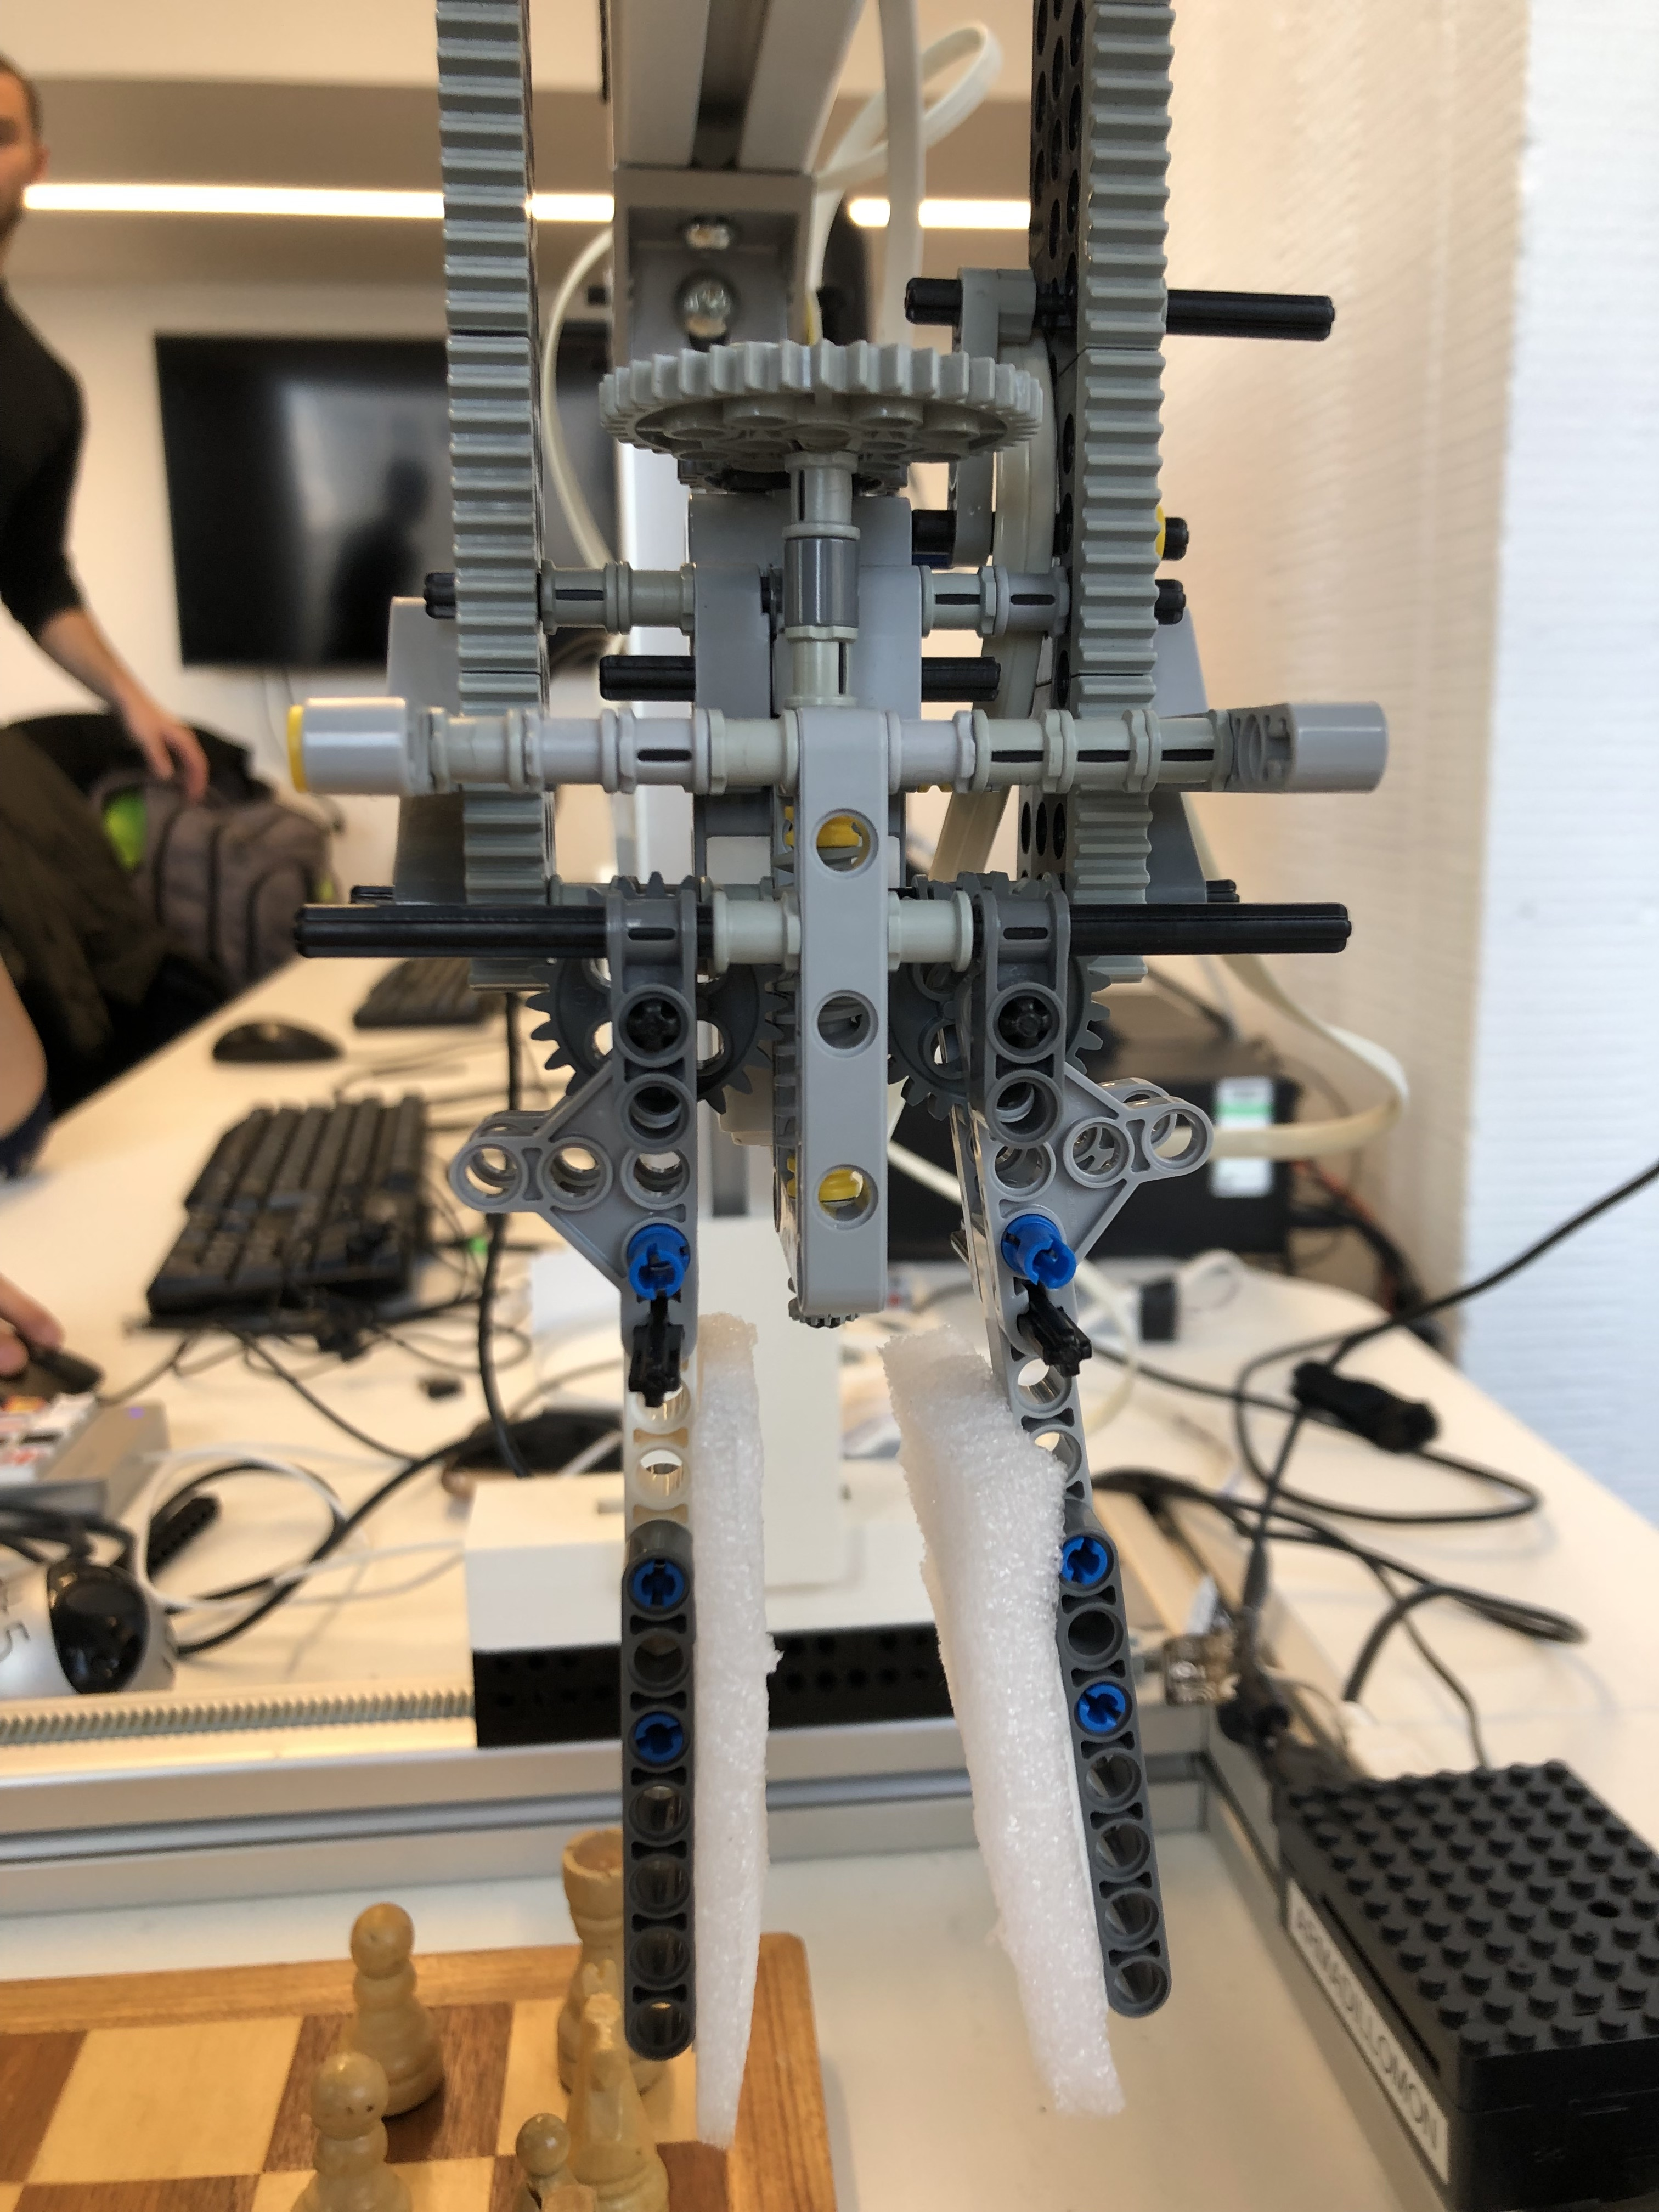
\includegraphics[scale = .05]{gripper}
   \captionof{figure}{Gripper}
   \label{fig:gripper}
%\end{figure}
\end{minipage}
\begin{minipage}[c]{.45\textwidth}
%\begin{figure}[h!]
  %\caption{Numpad}
  %\centering
  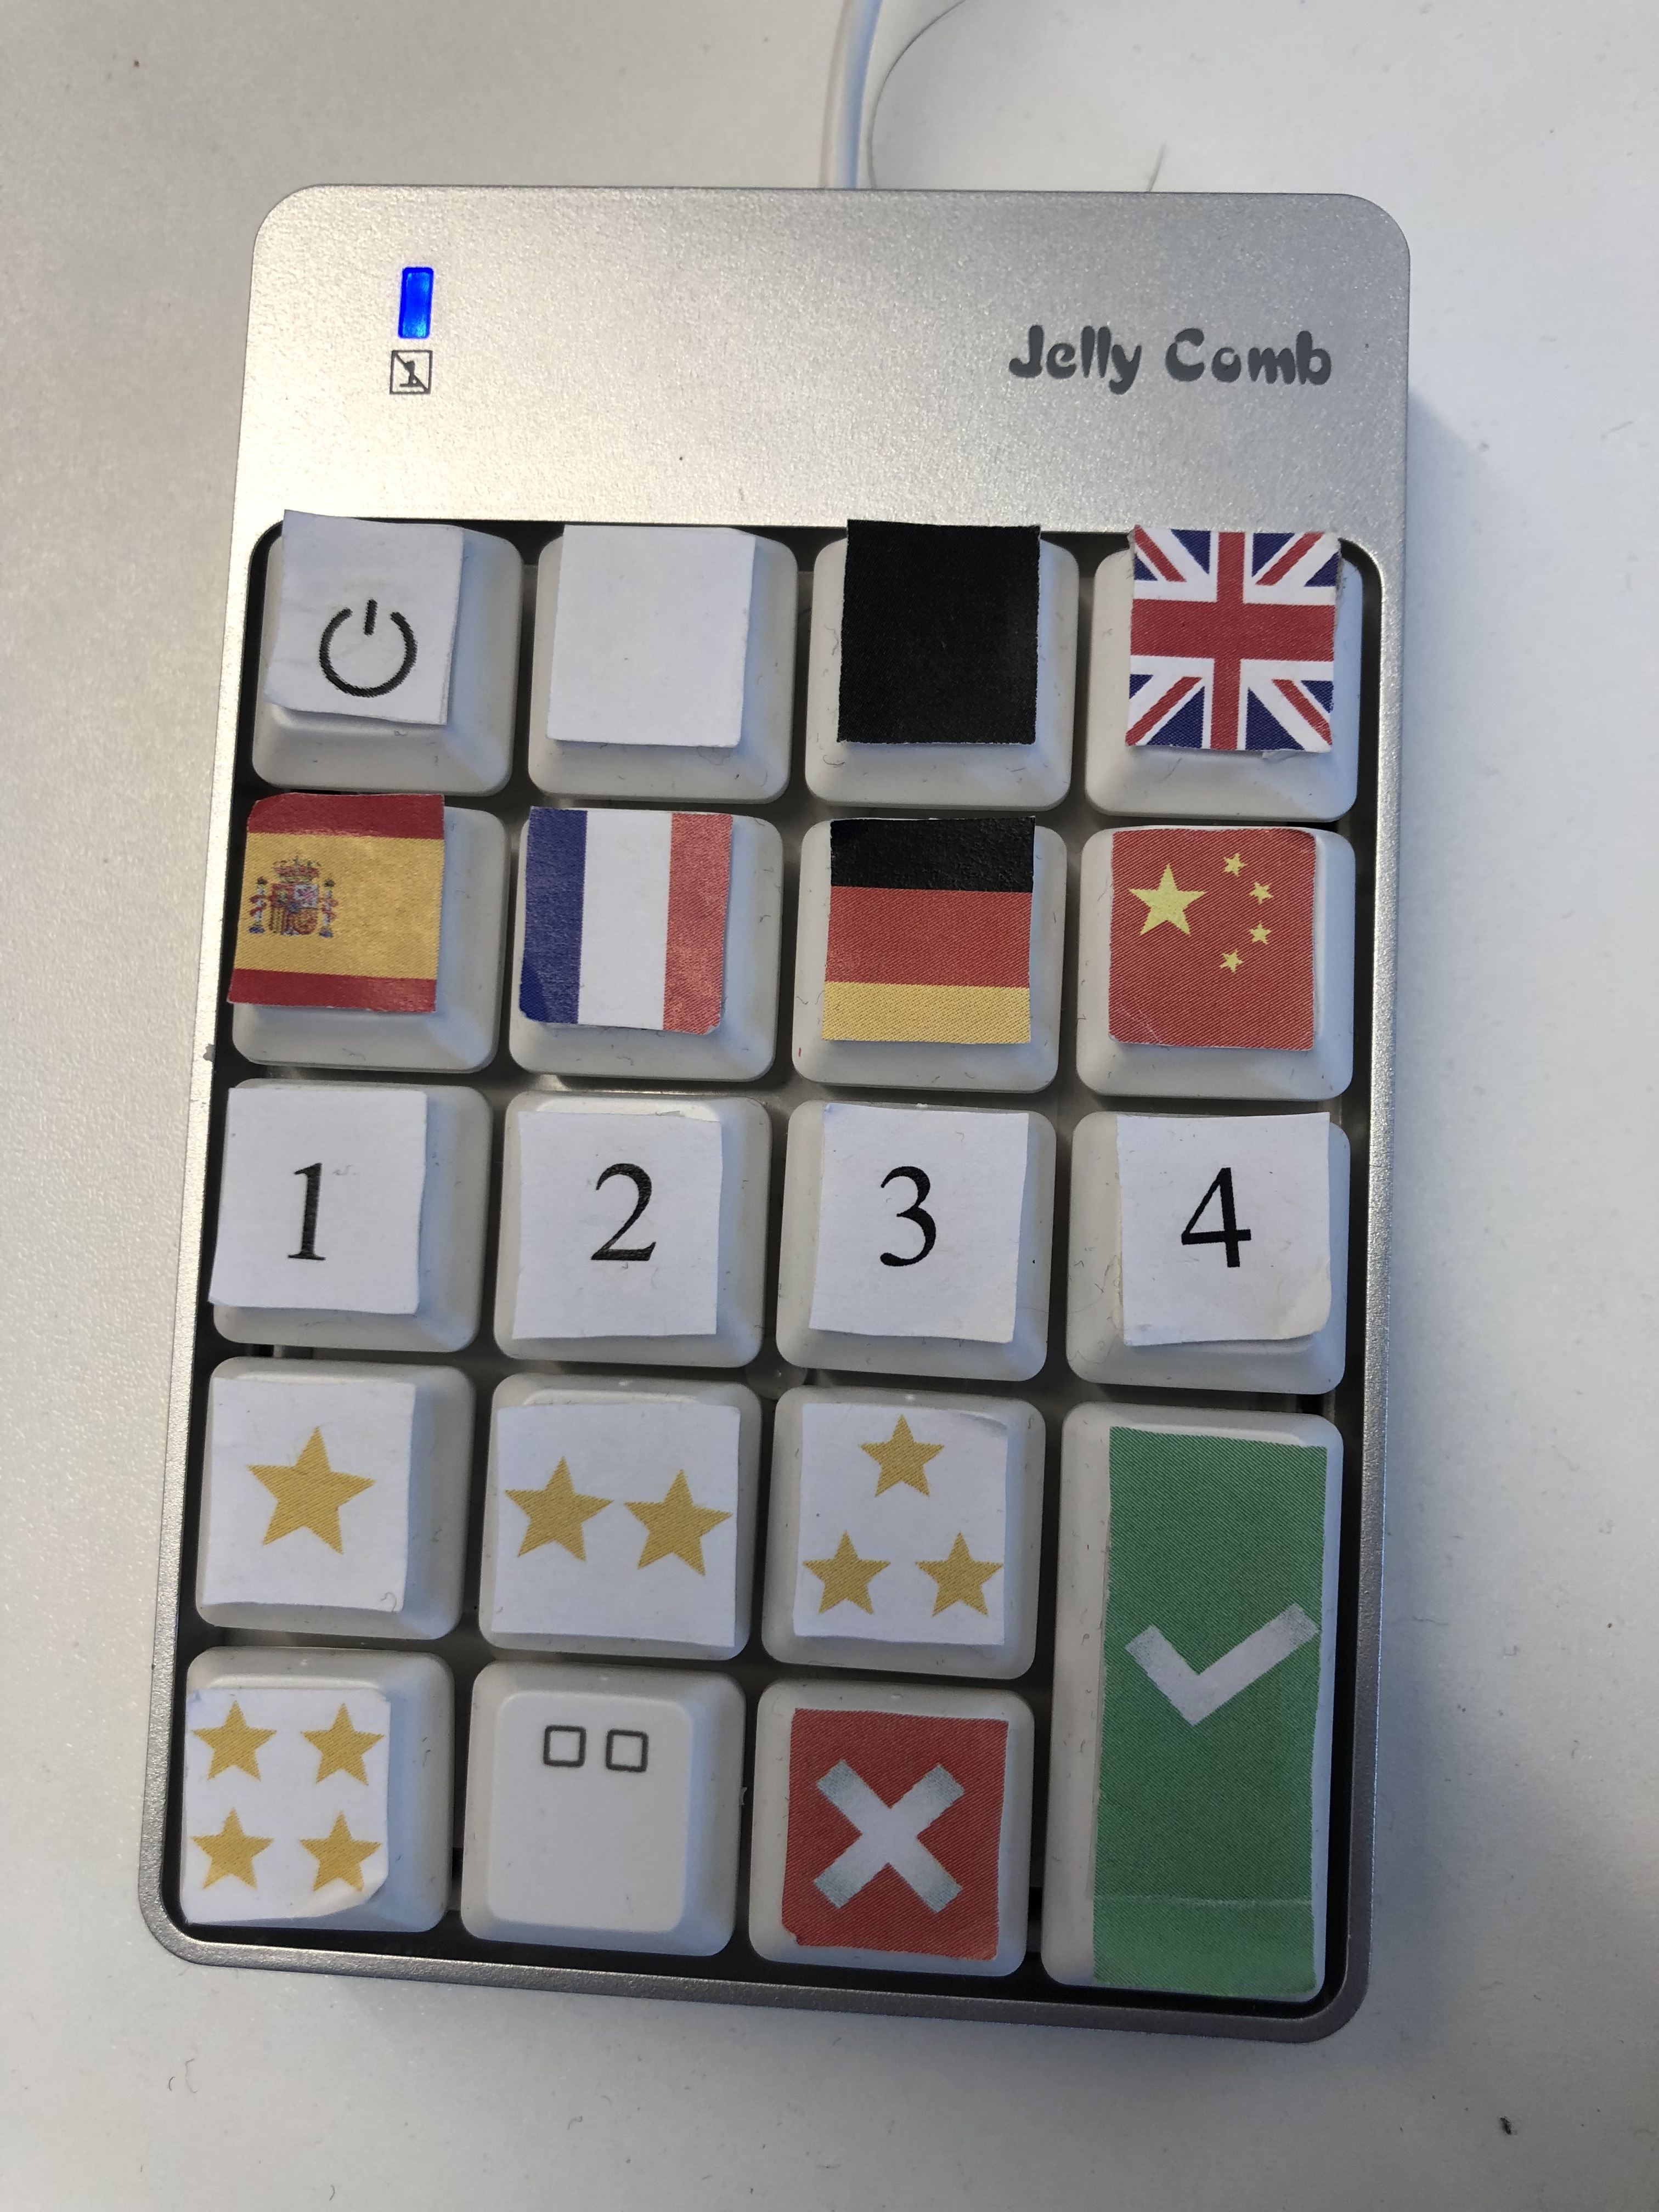
\includegraphics[scale = .05]{numpad}
   \captionof{figure}{Numpad}
   \label{fig:numpad}
%\end{figure}
\end{minipage}
\end{center}

\hspace{1cm}

\begin{center}
\begin{minipage}[c]{.5\textwidth}
%\begin{figure}[h!]
  %\caption{Entire Robot}
  \includegraphics[scale = .05]{Money.JPG}
   \captionof{figure}{Entire Robot}
   \label{fig:money}
%\end{figure}
\end{minipage}
\begin{minipage}[c]{.45\textwidth}
\begin{enumerate}
\item Aluminium alloy track with inlaid tracks.
\item 3D printed bases to hold the uprights. Motors situated along side these, to hold the uprights. 
\item Uprights. 
\item Chain suspended between gears on motors. The up-down movement is on this chain, so it can move left and right across the board. 
\item Up-down movement. Long lego strips held in place by the force of the gears pressing against tracks, and moved up and down by these gears moving along the tracks. 
\item Gripper. 
\end{enumerate}
\end{minipage}
\end{center}

\begin{figure}[h!]
  \caption{High Level Algorithm}
  \centering
  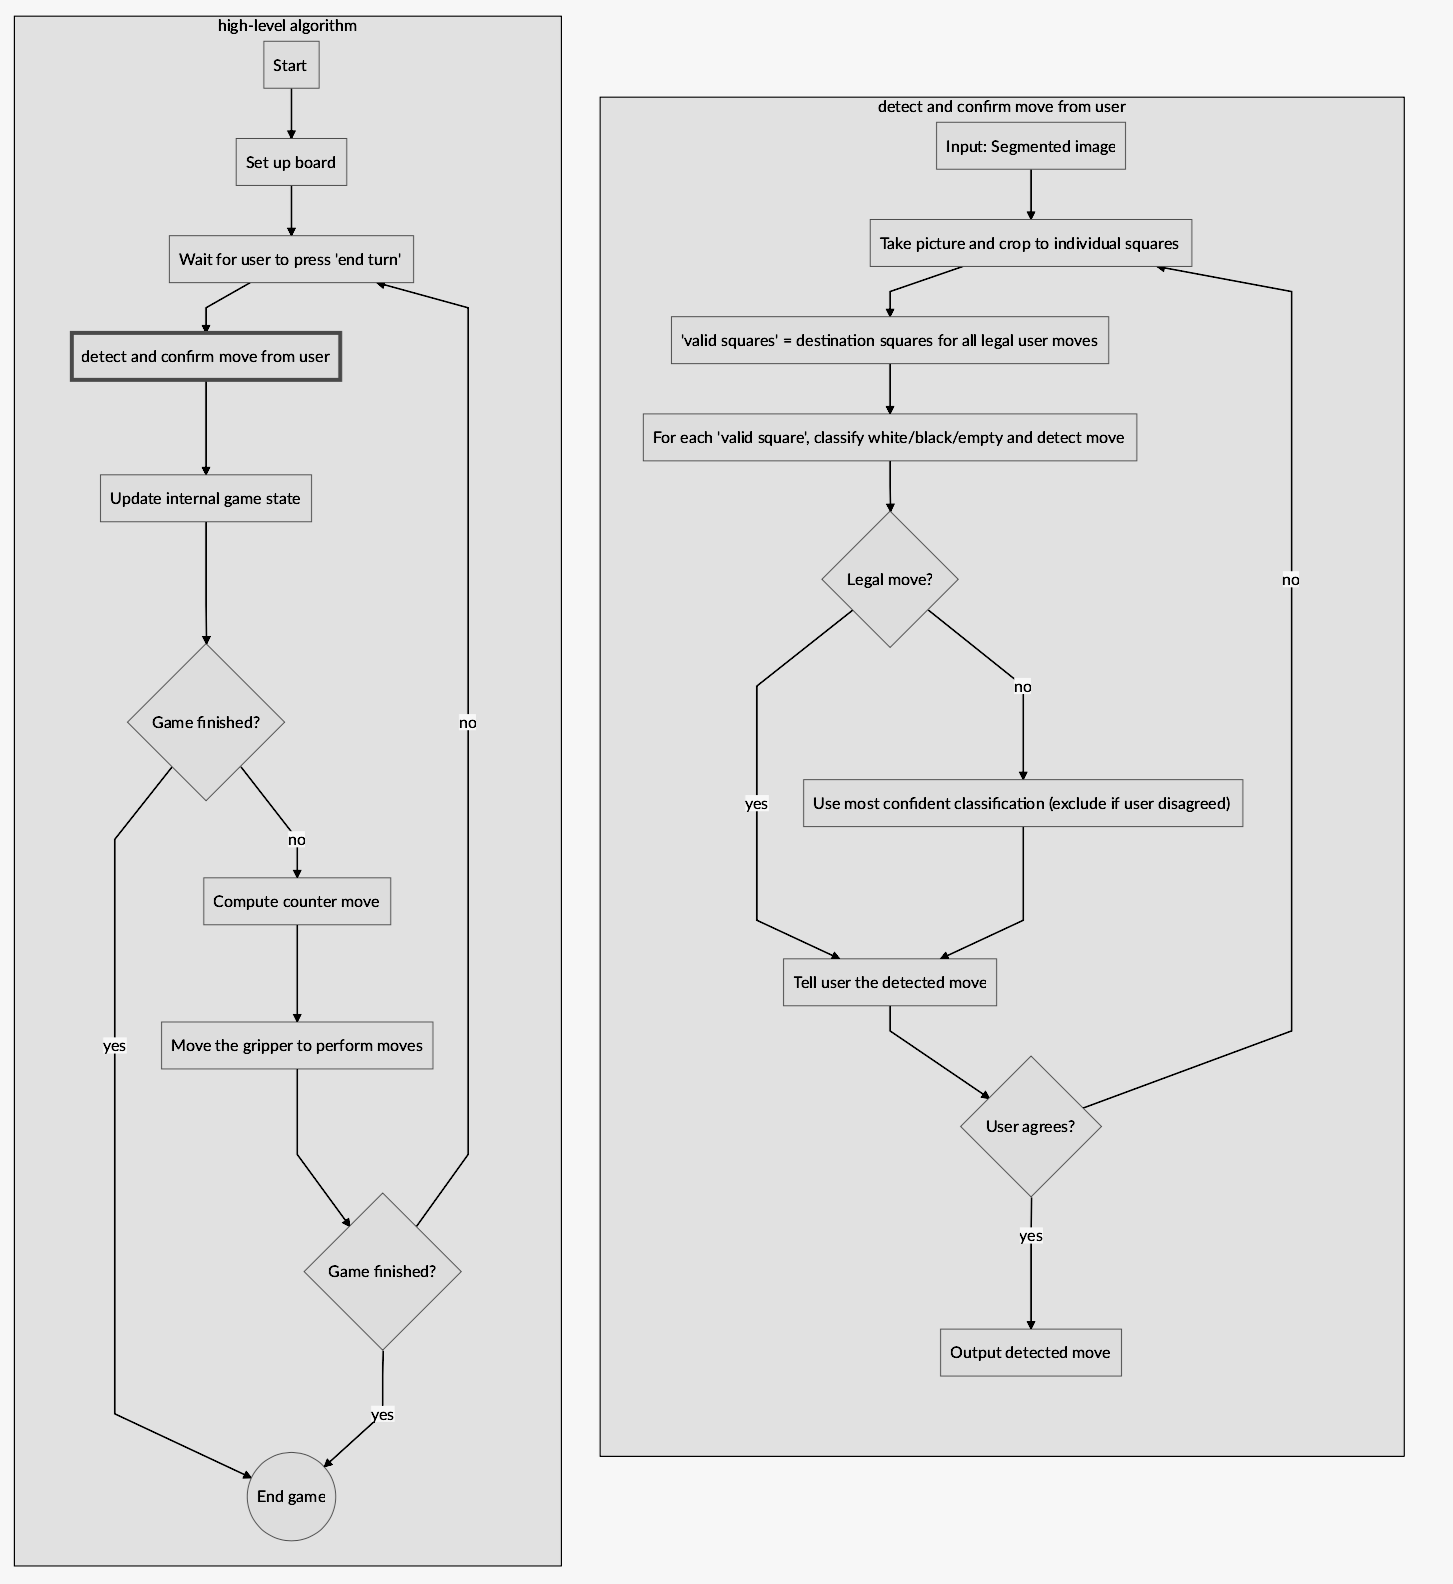
\includegraphics[scale = .3]{white_square.png}
\end{figure}

\pagebreak
\section{References}
\noindent [1] \href{https://www.ncbi.nlm.nih.gov/pmc/articles/PMC4734149/\#r63}{https://www.ncbi.nlm.nih.gov/pmc/articles/PMC4734149/\#r63} \newline
[2] \href{https://www.tandfonline.com/doi/abs/10.3109/07420520903523719?casa_token=xuj5yeT4EWEAAAAA\%3ADS5C1NhfiI1XBogq05OfmNmXPNALfdGdCkl8oOSUKUsNgLJZQW5dzziJ_a5yXX3H1YCVc57m8jc\&}{Burkhart Kimberly \& Phelps James R. (2009) AMBER LENSES TO BLOCK BLUE LIGHT AND IMPROVE SLEEP: A RANDOMIZED TRIAL, Chronobiology International, 26:8, 1602-1612, DOI: 10.3109/07420520903523719} \newline
[3] \href{http://www.mentalhealthamerica.net/blog/how-blue-light-affects-mental-health}{http://www.mentalhealthamerica.net/blog/how-blue-light-affects-mental-health} \newline
[4]\href{https://uk.rs-online.com/web/p/tubing-struts/7613322/}{https://uk.rs-online.com/web/p/tubing-struts/7613322/}\newline
[5]\href{https://stockfishchess.org/}{https://stockfishchess.org/}\newline
[6]\href{https://en.wikipedia.org/wiki/Forsyth\%E2\%80\%93Edwards\_ Notation}
{https://en.wikipedia.org/wiki/Forsyth\%E2\%80\%93Edwards\_ Notation}\newline
[7]\href{https://opencv.org/}{https://opencv.org/}



\end{document}
